%%%%%%%%%%%%%%%%%%%%%%%%%%%%%%%%%%%%%
% SECTION - ANÁLISIS DE SENTIMIENTO 
%%%%%%%%%%%%%%%%%%%%%%%%%%%%%%%%%%%%%

\section{Problema de Análisis de Sentimiento (Clasificación)}
\label{section-analisis-de-sentimiento}

%%%%%%%%%%%%%%%%%%%%%%%%%%%%%%%%%%%%%%%%%%%%%%%%%%%%%%%%%%%%%%%%%%%%%%%%%%%%%%%%%%%%%%%%%%%%%%%%%%%%%%%%%%%%%%%

\subsection{Descripción del problema}
\label{subsection-as-descripcion-problema}

El análisis de sentimiento es un subcampo del procesamiento de lenguaje natural que ha tenido un gran desarrollo en los últimos años. Este interés ha sido alimentado en gran parte por el auge de las redes sociales que ha dado lugar a la aparición de blogs, foros y aplicaciones en línea que le permiten a los usuarios discutir sobre cualquier tema y compartir sus opiniones. Este tipo de análisis es ampliamente usado por distintas empresas para entender la opinión de sus clientes y conocer la aceptación de sus productos y servicios. 

A través del análisis de sentimiento las empresas pueden estudiar los comentarios de los clientes para prestar una mejor atención, crear mejores productos o mejorar sus estrategias de marketing para atraer nuevos clientes. En líneas generales los resultados del análisis de sentimiento ayudan a conocer mejor los intereses y opiniones de los clientes sobre las tendencias del mercado.

El objetivo principal del problema es analizar una secuencia de texto y a partir de ella identificar o extraer información subjetiva que permita inferir si el sentimiento asociado a la frase es positivo o negativo. Desde otro punto de vista, se trata de una tarea de clasificación de la polaridad asociada a los textos que pueden estar presentes en documentos, oraciones u opiniones de forma masiva y automática. 

En el estudio de \cite{Bhavitha_sa}, los autores señalan que las técnicas de análisis de sentimientos se pueden clasificar en tres enfoques distintos en cuanto a la forma de solución.
\begin{enumerate}
  \item \textbf{Enfoque de aprendizaje automático:} Cuando utilizamos modelos de \textit{machine learning} en la solución del problema y generalmente nos basamos en un modelo especifico a partir del entrenamiento sobre un gran corpus de documentos.
  \item \textbf{Enfoque basados en léxico:} Mediante este enfoque, la orientación semántica de las palabras de un texto se calcula obteniendo las polaridades de las palabras a partir de un léxico predefinido. Es decir, habrá palabras en el texto que por si sola denotan ya una polaridad. Ejemplo, palabras como \textit{magnifico, bueno, grandioso, espectacular}, tienen un sentido positivo, mientras que palabras como \textit{horrible, malo, decepción}, tienen un significado negativo.
  \item \textbf{Enfoque híbrido:} Se basa en la combinación de información lingüística y estadística, reglas semánticas junto con el uso de redes neuronales profundas.
\end{enumerate}

Más recientemente, se utilizan técnicas de aprendizaje profundo, como BERT, T5 y GPT, para entrenar clasificadores de sentimientos de alto rendimiento que se evalúan mediante métricas como F1, recuperación y precisión. 

%%%%%%%%%%%%%%%%%%%%%%%%%%%%%%%%%%%%%%%%%%%%%%%%%%%%%%%%%%%%%%%%%%%%%%%%%%%%%%%%%%%%%%%%%%%%%%%%%%%%%%%%%%%%%%%

\subsection{Selección del Dataset}
\label{subsection-as-dataset-imdb}

Para evaluar los sistemas de análisis de sentimientos, se utilizan generalmente conjuntos de datos de referencia como:

\begin{itemize}
    \item \textbf{SST (Stanford Sentiment Treebank):} es un corpus con árboles de análisis sintáctico completamente etiquetados que permite un análisis completo de los efectos compositivos del sentimiento en el lenguaje. El corpus se basa en el conjunto de datos presentado por \citep{PANG_LEE_SST_https://doi.org/10.48550/arxiv.cs/0506075} y consta de 11.855 oraciones individuales extraídas de reseñas de películas. Se analizó con el analizador de Stanford e incluye un total de 215154 frases únicas de esos árboles de análisis, cada una anotada por 3 jueces humanos.
    Cada frase está etiquetada como negativa, algo negativa, neutral, algo positiva o positiva. El corpus con las 5 etiquetas se denomina SST-5 o SST de grano fino. Los experimentos de clasificación binaria en oraciones completas (negativas o algo negativas versus algo positivas o positivas con oraciones neutras descartadas) se refieren al conjunto de datos como SST-2 o SST binario.
    
     \item \textbf{GLUE (General Language Understanding Evaluation benchmark):} es una colección de nueve tareas de comprensión del lenguaje natural, que incluyen tareas de una sola oración CoLA y SST-2, tareas de similitud y paráfrasis MRPC, STS-B y QQP, y tareas de inferencia del lenguaje natural MNLI, QNLI, RTE y WNLI.
     
     \item \textbf{Large Movie Review Dataset IMDB:} es el conjunto de datos que se seleccionó para este experimento y que se procederá a describir a continuación.
\end{itemize}

El \textit{\textbf{Large Movie Review Dataset IMDB}} es un conjunto de datos con 50.000 reseñas de películas creado para la clasificación de sentimientos binarios que contiene sustancialmente más datos que los otros conjuntos de datos de referencia.

Como describen los creadores de este \textit{dataset} en su \textit{paper} del 2019 \textit{Learning Word Vectors for Sentiment Analysis} \cite{maas-EtAl:2011:ACL-HLT2011}, este conjunto de datos fue creado a partir de reseñas de películas realizadas por la audiencia y extraídas del sitio público IMDB. Para la construcción del mismo consideraron no incluir más de 30 reseñas por película.

Este conjunto de datos se encuentra balanceado, es decir, contiene un mismo número de reseñas positivas y negativas. Los autores para construirlo consideraron solo críticas altamente polarizadas en base al sistema de rating que tiene IMDB y de esa forma consideraron una crítica negativa a aquellas reseñan que tenían una puntuación $\leq$ 4 sobre 10 y positiva si la puntuación era $\geq$ 7 sobre 10. Las reseñas neutrales no fueron incluidas

Para el propósito de este trabajo se usó una versión del \textit{dataset} original transformado y disponible en la plataforma \textit{kaggle.com} \citep{n_2019}. Esta versión ha sido transformada a un archivo de valores separados por comas, CSV (del inglés comma-separated values), en el cual se presentan dos columnas una para la reseña y otra para el sentimiento.

La razón por la que se escogió este \textit{dataset} y no otro es la amplia cantidad de soluciones desarrolladas tomando como base de entrenamiento el mismo, esto permitirá poder hacer un estudio del resultado obtenido y compararlo con otros modelos.

%%%%%%%%%%%%%%%%%%%%%%%%%%%%%%%%%%%%%%%%%%%%%%%%%%%%%%%%%%%%%%%%%%%%%%%%%%%%%%%%%%%%%%%%%%%%%%%%%%%%%%%%%%%%%%%

\subsection{Estado del arte}
\label{subsection-as-estado-del-arte}

Para evaluar el estado del arte relacionado a la solución de análisis de sentimiento sobre el \textit{dataset} de reseñas de IMDB se utilizaron diversas fuentes. 

En el trabajo de \cite{Dang_2020} los autores analizaron y realizaron una comparación entre distintos estudios que usan el aprendizaje profundo como las \acrlong{acr_dnn} (\acrshort{acr_dnn}, por sus siglas en inglés), \acrlong{acr_rnn} (\acrshort{acr_rnn}, por sus siglas en inglés) y \acrlong{acr_cnn} (\acrshort{acr_cnn}, por sus siglas en inglés), para resolver diferentes problemas asociados al análisis de sentimiento. En este estudio no se incluyeron las recién aparecidas (para ese momento) redes basadas en Transformers. Los autores usaron distintos datasets para la evaluación entre ellos el mismo utilizado en este trabajo \ref{subsection-as-dataset-imdb} y utilizaron en el preprocesamiento de los datos dos técnicas distintas de procesamiento de texto (\gls{gls_wordembeddings} y \gls{gls_tfidf}). En sus conclusiones, los autores deducen una fiabilidad ligeramente superior en la mayoría de conjunto de datos con las redes neuronales recurrentes, sin embargo, igual mencionan un tiempo de cálculo mucho más largo, como se puede evidenciar en las imágenes \ref{fig-as-eda-accuracy-comparison} y \ref{fig-as-eda-cpu-comparison} 

\begin{figure}[ht!]
    \centering
    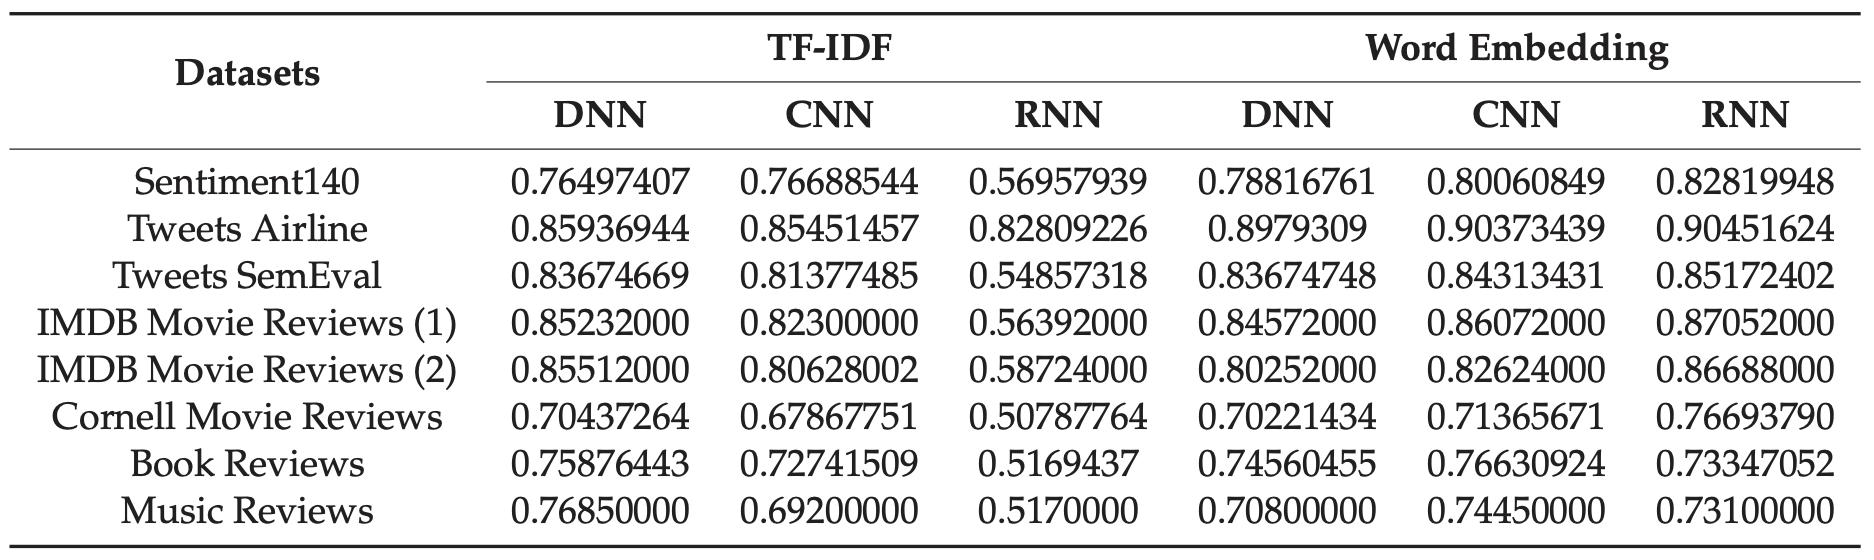
\includegraphics[scale=0.45]{figuras/as-eda-accuracy-comparison.png}
    % \caption[Así aparece el rótulo en el índice]{Así aparece el rótulo en el texto.}
    \caption[Análisis de Sentimiento - Tabla - Accuracy]{Comparación del accuracy obtenido para datasets con dos clases (positivo y negativo), en el artículo \textit{Sentiment Analysis Based on Deep Learning: A Comparative Study}. \textbf{Fuente: \cite{Dang_2020}}}
    \label{fig-as-eda-accuracy-comparison}
\end{figure}

\begin{figure}[ht!]
    \centering
    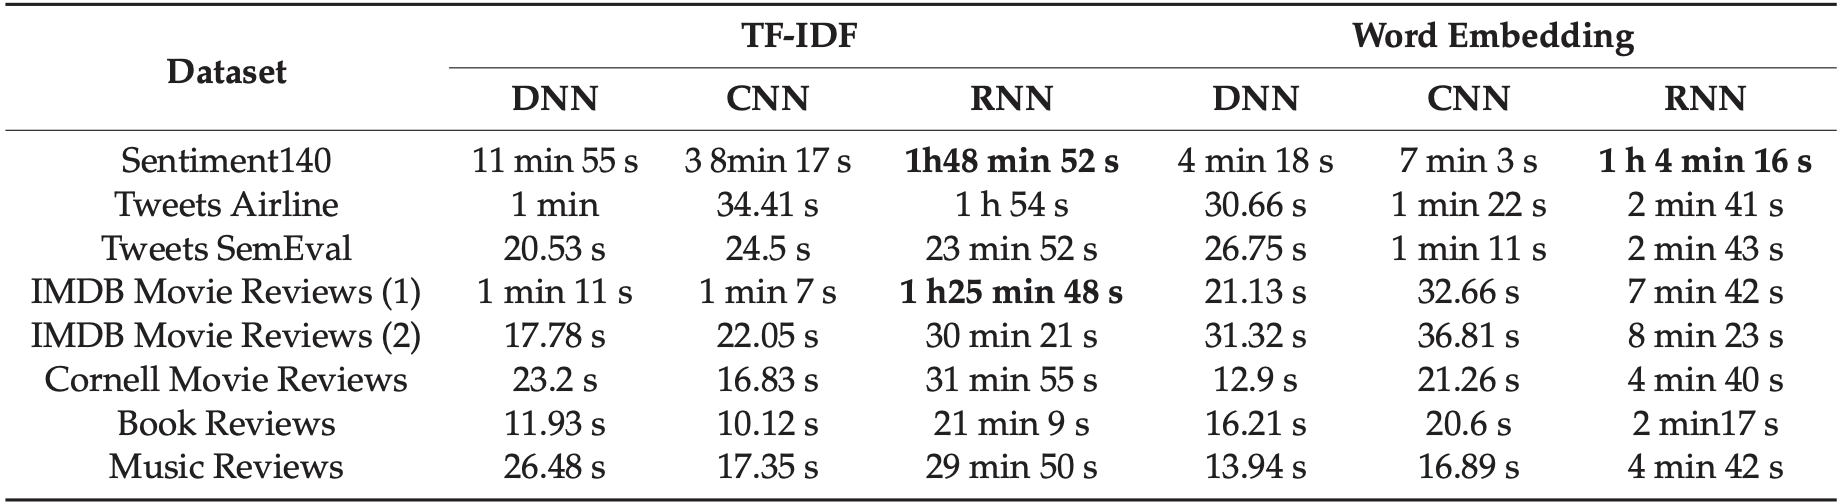
\includegraphics[scale=0.45]{figuras/as-eda-cpu-comparison.png}
    % \caption[Así aparece el rótulo en el índice]{Así aparece el rótulo en el texto.}
    \caption[Análisis de Sentimiento - Tabla - Performance]{\textbf{Comparación de los tiempos de cómputo experimentados para el entrenamiento de modelos con \acrshort{acr_gpu}, en el artículo \textit{Sentiment Analysis Based on Deep Learning: A Comparative Study}. Fuente: \cite{Dang_2020}}}
    \label{fig-as-eda-cpu-comparison}
\end{figure}

Es importante mencionar con respecto a este estudio que si bien las RNN evidenciaron tener un mejor desempeño con todos los datasets esto solo ocurrió con el uso de Word Embedding como técnica de preprocesado de los datos y no con \gls{gls_tfidf}.

Adicionalmente nos basamos en el sitio web NLP-progress (\url{https://nlpprogress.com/}) \cite{Ruder_NLP-progress_2022}, el cual es un repositorio en linea que hace un seguimiento del progreso en distintos problemas en el procesamiento del lenguaje natural NLP, incluidos los datasets y el estado del arte actual para las tareas de NLP más comunes.

Este repositorio muestra un ranking de modelos \ref{tbl-nlpprogress-ranking} que resuelven el problema de análisis de sentimiento haciendo uso del dataset de IMDB \ref{subsection-as-dataset-imdb}. En este ranking dos de los primeros tres modelos están basados en una implementación de BERT descrita por  \cite{FTBERTCLAS_https://doi.org/10.48550/arxiv.1905.05583} en su \textit{paper} ``\textit{How to Fine-Tune BERT for Text Classification?}'', y el modelo que presenta el mejor performance, XLNet \cite{XLNET_https://doi.org/10.48550/arxiv.1906.08237} es un método de preentrenamiento autorregresivo generalizado similar a BERT que permite aprender contextos bidireccionales mediante la maximización de la probabilidad esperada de todas las permutaciones del orden de factorización.

\begin{table}[ht!]
\resizebox{\textwidth}{!}{
\begin{tabular}{l|c|l}
\toprule
\textbf{Modelo} & \textbf{Accuracy} & \textbf{Paper} \\ \midrule
XLNet \cite{XLNET_https://doi.org/10.48550/arxiv.1906.08237}                    & 96.21     & XLNet: Generalized Autoregressive Pretraining for Language Understanding  \\ \midrule
BERT\_large+ITPT \cite{FTBERTCLAS_https://doi.org/10.48550/arxiv.1905.05583}    & 95.79     & How to Fine-Tune BERT for Text Classification?                            \\ \midrule
BERT\_base+ITPT  \cite{FTBERTCLAS_https://doi.org/10.48550/arxiv.1905.05583}    & 95.63     & How to Fine-Tune BERT for Text Classification?                            \\ \bottomrule
\end{tabular}
}
% \caption[Así aparece el rótulo en el índice]{Así aparece el rótulo en el texto.}
\caption[Análisis de Sentimiento - Ranking de modelos según NLPProgress]{\textbf{Ranking de modelos según NLPProgress (\url{http://nlpprogress.com/english/sentiment_analysis.html}) en la resolución de la tarea de análisis de sentimiento. Fuente NLPProgress}}
\label{tbl-nlpprogress-ranking}
\end{table}

Y por último citamos el ranking de otro reconocido sitio web \textit{Papers with Code} (\url{https://paperswithcode.com/}), el cual es un recurso de referencia para \textit{papers} científicos que representan el más actual estado del arte en distintas casuísticas del \textit{machine learning}. La plataforma está compuesta de casi 5.000 benchmarks, 2.300 tareas y 50.000 \textit{papers} que permiten comparar distintos enfoques en la resolución de distintos problemas.

Particularmente para el análisis de sentimiento sobre el dataset de IMDB, la plataforma compara distintas investigaciones rankeadas según el accuracy obtenido con este conjunto de datos. Es interesante observar que entre las 10 mejores soluciones encontramos 7 trabajos basados en Transformers y la mitad de ellos son modelos basados en BERT. (ver figura \ref{fig-as-eda-pwc-table})

\begin{figure}[ht!]
    \centering
    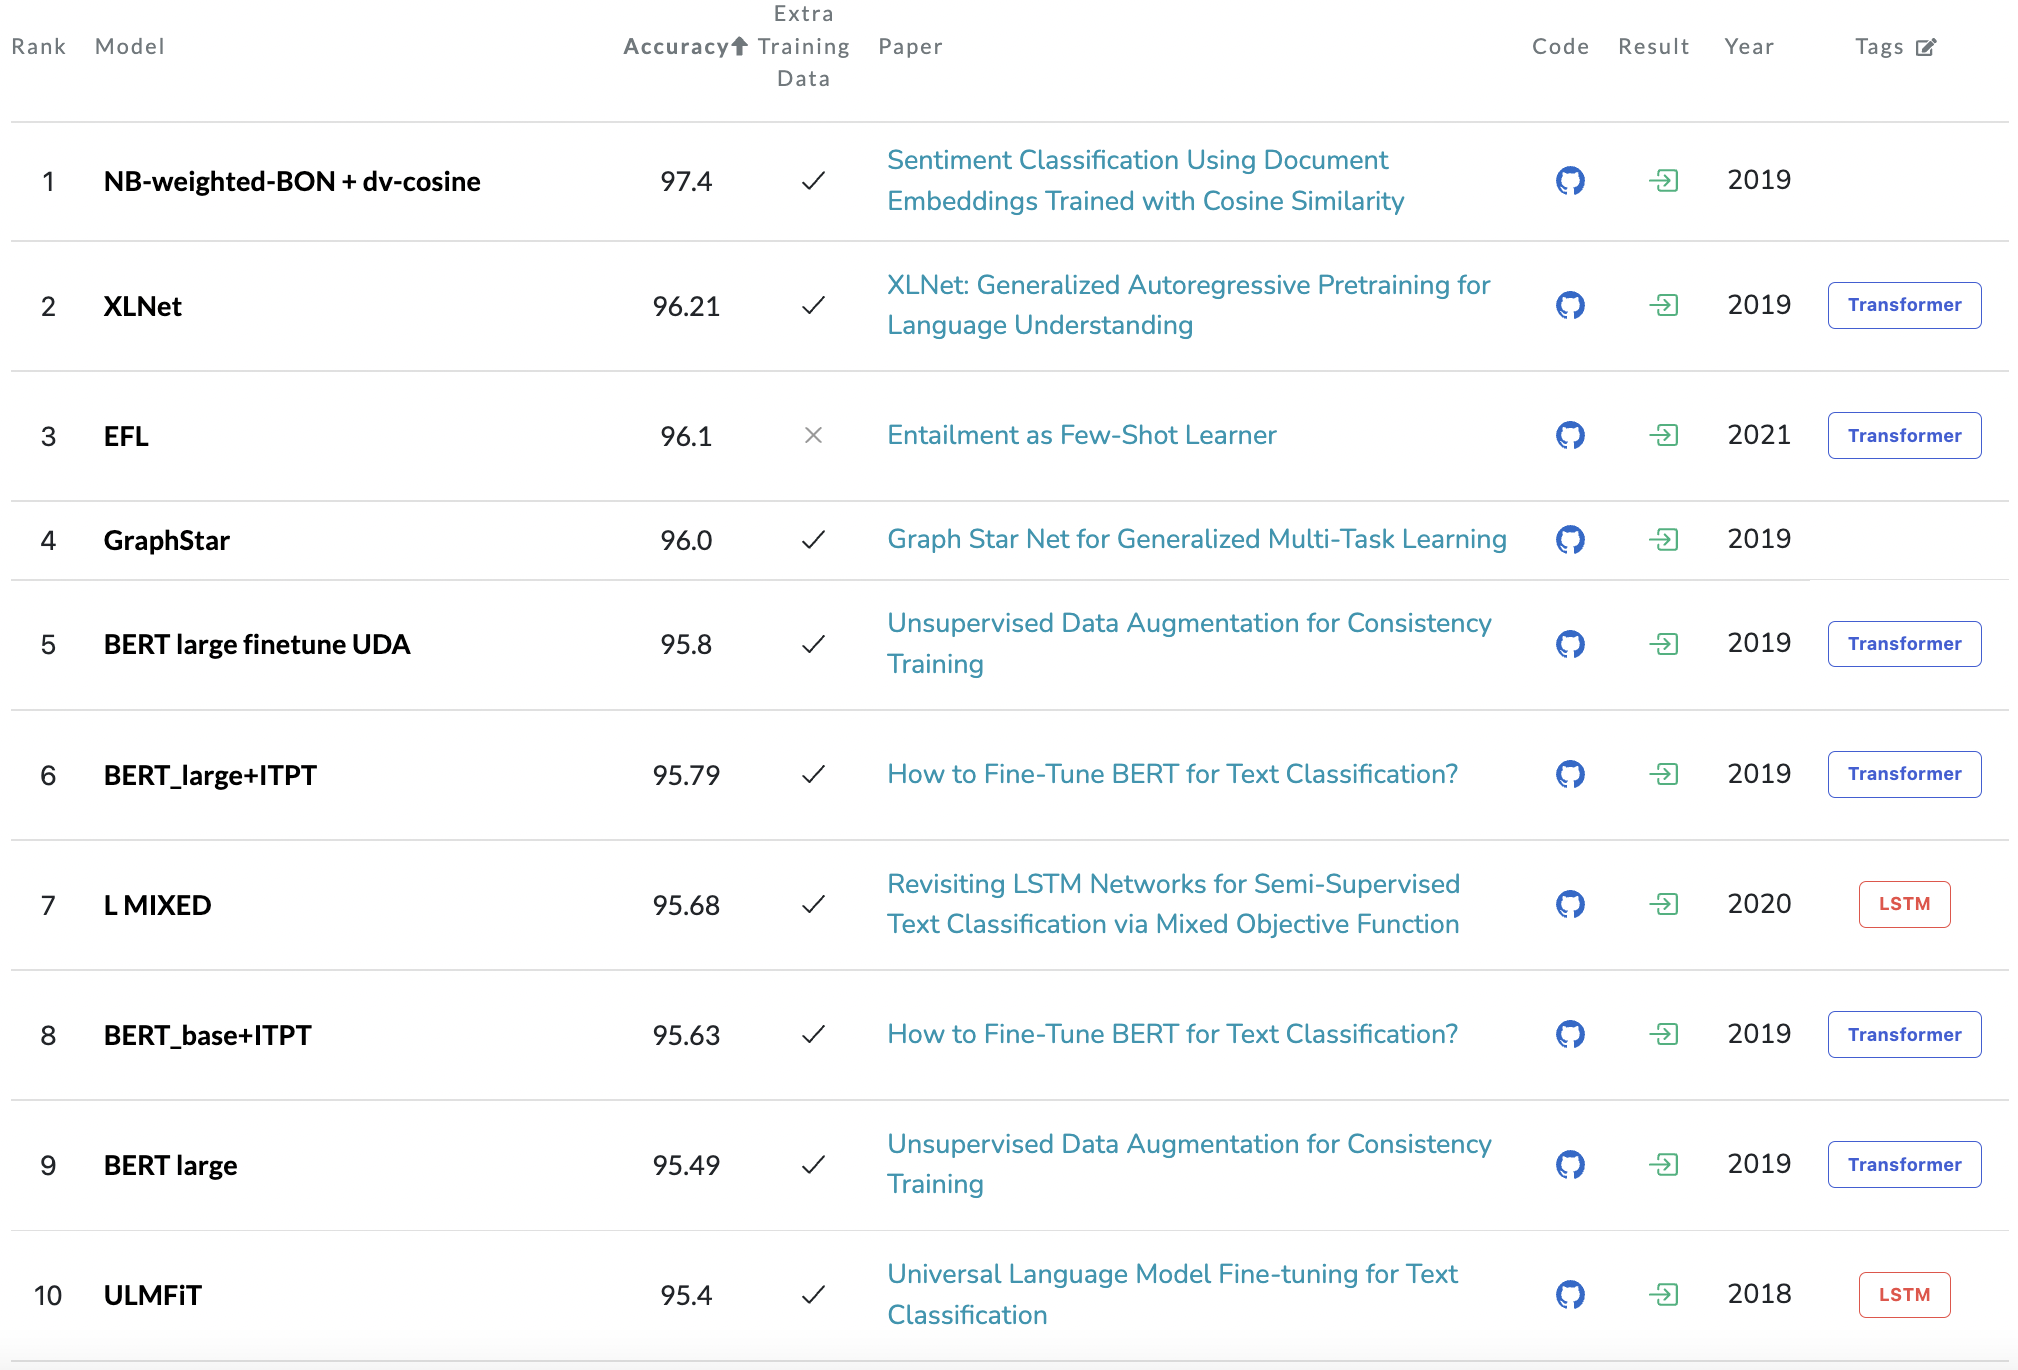
\includegraphics[scale=0.4]{figuras/as-eda-pwc-table.png}
    % \caption[Así aparece el rótulo en el índice]{Así aparece el rótulo en el texto.}
    \caption[Análisis de Sentimiento - Papers with code - Top 10]{\textbf{Esta imagen muestra el ranking de modelos organizados por el accuracy obtenido en el problema de análisis de sentimiento sobre el dataset de reseñas de IMDB. En este ranking podemos ver 7 modelos basados en transformers y la mitad de los modelos en el top 10 son modelos basados en BERT. Fuente: \url{https://paperswithcode.com/sota/sentiment-analysis-on-imdb}}}
    \label{fig-as-eda-pwc-table}
\end{figure}

%%%%%%%%%%%%%%%%%%%%%%%%%%%%%%%%%%%%%%%%%%%%%%%%%%%%%%%%%%%%%%%%%%%%%%%%%%%%%%%%%%%%%%%%%%%%%%%%%%%%%%%%%%%%%%%

\subsection{Arquitectura de la solución}
\label{subsection-as-arquitectura-de-la-solucion}
Como se mencionó anteriormente en la sección \ref{subsection-arquitectura-bert}, la arquitectura de BERT ha sido diseñada para adaptarse a la resolución de distintos problemas a través de un leve ajuste. Este caso en particular se trata de un problema de clasificación de una frase en dos clases objetivos, en otras palabras, dada una frase clasificarla como sentimiento positivo o sentimiento negativo.

La forma de afrontar un problema de clasificación con BERT es en base al token especial [CLS]. Como indican los autores en el \textit{paper} de BERT, ``El primer token de cada secuencia es siempre un token de clasificación especial [CLS]. El estado oculto final correspondiente a este token se utiliza como representación de secuencia agregada para tareas de clasificación."  (\cite{https://doi.org/10.48550/arxiv.1810.04805})

En la imagen \ref{fig-bert-as-architecture} se describe la arquitectura general de la solución propuesta para este problema, donde podemos observar las 12 capas de Transformer que componen el modelo. Cada una de estas capas toma un \textit{embedding} de tokens como entrada y produce la misma cantidad de \textit{embeddings} en la salida. En la salida del último Transformer se construye un clasificador a través del primer \textit{embedding} correspondiente al token [CLS].

\begin{figure}[ht!]
    \centering
    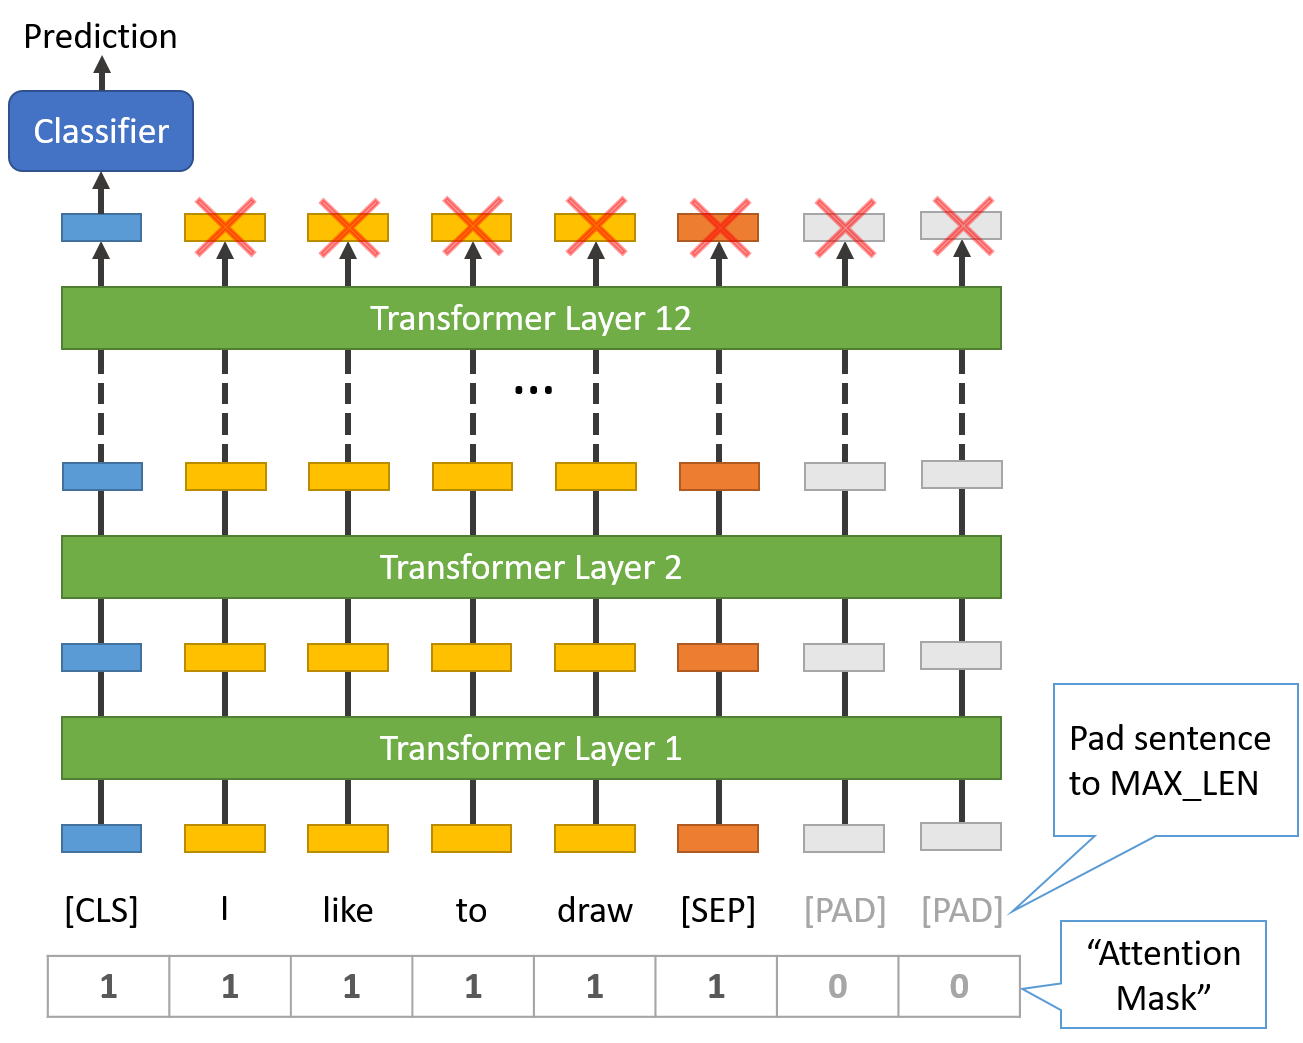
\includegraphics[scale=0.5]{figuras/bert-as-architecture.png}
    % \caption[Así aparece el rótulo en el índice]{Así aparece el rótulo en el texto.}
    \caption[Análisis de Sentimiento - Arquitectura de la solución]{\textbf{Adecuación de la arquitectura de BERT para la solución de problemas de clasificación basados en una frase de entrada. Fuente: \cite{chris_mccormick_and_nick_ryan_bert_2019}}}
    \label{fig-bert-as-architecture}
\end{figure}

%%%%%%%%%%%%%%%%%%%%%%%%%%%%%%%%%%%%%%%%%%%%%%%%%%%%%%%%%%%%%%%%%%%%%%%%%%%%%%%%%%%%%%%%%%%%%%%%%%%%%%%%%%%%%%%

\subsection{Preparación de los datos}
\label{as-preparacion-de-los-datos}

Durante el proceso de preparación de los datos se abordaron dos etapas. La primera de ellas de exploración y saneamiento de los datos. Durante esta primera etapa:

\begin{itemize}
    \item Se identificó y valido que tal como indica la documentación \cite{maas-EtAl:2011:ACL-HLT2011}, el dataset está compuesto por 50000 registros bien balanceados (25000 datos etiquetados como positivos y 25000 datos etiquetados como negativos) como se pudo confirmar una vez fueron cargados los datos. 
    \item Se pudo notar que ciertos registros se encontraban duplicados. Estos registros duplicados fueron removidos.
    \item Se creó y aplicó una función de limpieza que permite para cada una de las reseñas limpiar algunos elementos que podrían causar ruido y carecen de valor en el análisis y entrenamiento del modelo como las etiquetas \acrshort{acr_html}, texto entre corchetes y algunos signos de puntuación.
\end{itemize}

La segunda etapa se basó en un proceso de normalización de los datos de entrada para BERT. Al tratarse BERT de un modelo preentrenado, este espera que los datos de entrada tengan un formato especifico, tal como se indica en la sección \ref{subsection-bert-finetunning}. La normalización de los datos de entrada se basa en la construcción adecuada de los \textit{embeddings} para que el modelo pueda entender cada una de las sentencias de entrada, esto consiste en:

\begin{enumerate}
    \item Como se describe en la arquitectura de la solución (ver figura \ref{fig-bert-as-architecture}), el modelo de BERT tiene dos restricciones:
    \begin{enumerate}
    \item Todas las sentencias de entrada deben tener la misma longitud, por ese motivo las sentencias son truncadas o rellenadas con un token especial denominado [PAD]
    \item La longitud máxima de la sentencia de entrada es de 512 tokens.
    \end{enumerate}
    Al tener sentencias de entrada de longitud variable se optó en este caso por truncar los datos de entrada a una longitud máxima de 512 tokens. En otras palabras estamos basando el entrenamiento en los primeros 512 tokens de cada reseña, desechando el resto de la información. 
    \item Añadir sentencias de entrada que tengan agregados los tokens especiales al comienzo y al final de cada sentencia.
    \begin{enumerate}
    \item El token [SEP] es un token especial que se utiliza para demarcar el fin de una sentencia o la separación entre dos sentencias. En este caso se utiliza como delimitador final de la única sentencia de entrada.
    \item El token [CLS] se debe anteponer a cada sentencia de entrada. Este token es usado en las tareas de clasificación, pero indistintamente del problema a resolver el modelo BERT siempre espera recibirlo como el comienzo de la entrada. La importancia de este token radica en que actúa como una representación agregada para las atareas de clasificación. La última capa oculta de este token se usa como una representación de la sentencia para la clasificación de secuencias.
    \end{enumerate}
    \item Agregar dos embeddings de información para el modelo:
    Al embedding de tokens producto del tokenizador de BERT (Token IDs), se deben agregar dos \textit{embeddings} adicionales:
    \begin{enumerate}
    \item Mask IDs o máscara de atención que diferencia cuales elementos de la secuencia son tokens y cuales son tokens de relleno o padding. Se trata simplemente una matriz de 1s y 0s que indica qué tokens están rellenando y cuáles no. Esta máscara le dice al mecanismo de auto-atención en BERT que no incorpore estos tokens [PAD] en su interpretación de la sentencia.
    \item Segment IDs usado para distinguir diferentes sentencias. En este caso en el que tenemos una sola sentencia se trata de un vector de 0s.
    \end{enumerate}
\end{enumerate}

Adicionalmente es importante mencionar que existen técnicas y trabajos enfocados en cómo manejar la limitación que presenta BERT en cuanto a la extinción de los tokens de la secuencia de entrada. 

Existen tres enfoques distintos basados en el costo computacional:
\begin{itemize}
    \item \textbf{Bajo costo computacional:} Seleccionar una parte del texto original. Los ejemplos incluyen elegir los primeros n tokens, los últimos n tokens o compilar una nueva instancia de texto a partir del principio y el final de la instancia de texto original.
    \item \textbf{Costo computacional medio a alto:} Usar modelos de Transformers recientes (como Longformer) que tienen un límite de 4096 tokens en lugar de 512. Estos nuevos métodos tienen mecanismos de atención modificados que reducen el costo computacional.
    \item \textbf{Alto costo computacional:} Dividir la instancia de texto en fragmentos que se ajusten a un modelo como BERT con un límite estándar de 512 tokens por instancia e implementar el modelo en cada parte por separado, luego unir las representaciones vectoriales resultantes.
\end{itemize}

En el artículo de \cite{Fiok_2021_TextGuideLong} además de proponer un nuevo método llamado Text Guide, que es un método de bajo coste computacional el cual pretende hacer un truncamiento mas inteligente de la instancia de entrada.

Por último mencionar que \cite{FTBERTCLAS_https://doi.org/10.48550/arxiv.1905.05583} en su \textit{paper} hace una comparación usando distintas técnicas para truncar el texto, tomando en algunos casos el principio, en otros casos el final y en algunos casos haciendo combinaciones de distintos segmentos del texto. De este trabajo igual podemos concluir que la diferencia del performance del modelo no es significativa entre las distintas técnicas. 

Por las razones antes expuestas y entendiendo que el m´todo elegido no impactará mucho el performance del modelo,  para este trabajo se decidió utilizar un truncamiento simple tomando los primeros 512 tokens de la sentencia de entrada.


%%%%%%%%%%%%%%%%%%%%%%%%%%%%%%%%%%%%%%%%%%%%%%%%%%%%%%%%%%%%%%%%%%%%%%%%%%%%%%%%%%%%%%%%%%%%%%%%%%%%%%%%%%%%%%%

\subsection{Modelo y Fine Tuning}
\label{as-finetunning}

El modelo de BERT se obtuvo desde Tensorflow Hub (\url{https://www.tensorflow.org/hub}). TensorFlow Hub es un repositorio de modelos de aprendizaje automático preentrenados, listos para poder implementar un fine-tunning.

Se usó como modelo BERT preentrenado la versión bert\_multi\_cased\_L-12\_H-768\_A-12. Para hacer el clasificador se optó por usar el API Keras de Tensorflow tomando las salidas del modelo de BERT, específicamente el pooled\_output (embedding del token [CLS]) y creando una capa única para la tarea de clasificación, para ayudar a prevenir el sobreajuste se hizo un droput de 10\%. En esta última capa, se aplica la función softmax para obtener las probabilidades predichas del modelo entrenado.

Para entrenar el modelo propuesto se utilizo como valores de los hiperparámetros los recomendados en el \textit{paper} de BERT. Según los autores del \textit{paper} BERT no necesita muchas epocas para ser entrenado y recomiendan que sean entre 2 y 4. \cite{https://doi.org/10.48550/arxiv.1810.04805}:

\begin{itemize}
    \item Tamaño del lote = 8
    \item Tasa de aprendizaje = 2e-5
    \item Longitud máxima de secuencia = 512
    \item Épocas = 3
\end{itemize}

\begin{figure}[ht!]
    \centering
    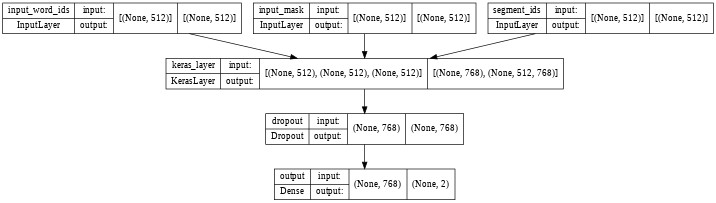
\includegraphics[scale=0.6]{figuras/as-modelo.png}
    % \caption[Así aparece el rótulo en el índice]{Así aparece el rótulo en el texto.}
    \caption[Análisis de Sentimiento - Modelo de la solución]{\textbf{Modelo de BERT propuesto para la solución de este problema de clasificación. En el modelo se observan como entrada las tres embeddings que la conforman, el token embedding, el de segmentación y el posicional, estos van directamente a la capa preentrenada de BERT, luego se agrega una capa de dropout y una última capa que recibe el dropout del embedding del token [CLS] y como salida tiene solo dos neuronas, una para cada clase a predecir. Fuente: Imagen propia}}
    \label{fig-as-modelo}
\end{figure}

El entrenamiento se realizó usando Google Colab y utilizando la GPU (Graphic Processing Unit). La duración del entrenamiento ha sido:

\begin{itemize}
    \item Primera Época = 3368 segundos.
    \item Segunda Época = 3373 segundos. 
    \item Tercera Época = 3372 segundos.
    \item Entrenamiento total = 10113 segundos, aproximadamente 2 horas y 50 minutos.
\end{itemize}

El código fuente del entrenamiento se encuentra en el repositorio Github \url{https://github.com/lsizaguirre/09MIAR-TFM}

%%%%%%%%%%%%%%%%%%%%%%%%%%%%%%%%%%%%%%%%%%%%%%%%%%%%%%%%%%%%%%%%%%%%%%%%%%%%%%%%%%%%%%%%%%%%%%%%%%%%%%%%%%%%%%%

\subsection{Resultados y Conclusiones.}
\label{as-resultados-y-conclusiones}

Podemos observar que con una configuración de red muy sencilla y con los parámetros recomendados para el fine-tunning se obtienen resultados bastante buenos y cercanos a los que definen el estado del arte. Se podría intentar hacer un ajuste más sofisticado y con ello obtener mejores resultados.

Las siguientes imágenes muestran algunas de las métricas obtenidas durante la evaluación del experimento.

\begin{figure}[ht!]
    \centering
    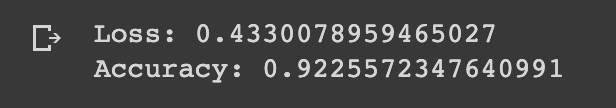
\includegraphics[scale=0.6]{figuras/as-resultados-1.png}
    % \caption[Así aparece el rótulo en el índice]{Así aparece el rótulo en el texto.}
    \caption[Análisis de Sentimiento - Resultados - Accuracy y Loss]{\textbf{Accuracy y Loss obtenidos con el modelo. Fuente: Imagen propia}}
    \label{fig-as-resultados-1}
\end{figure}

\begin{figure}[ht!]
    \centering
    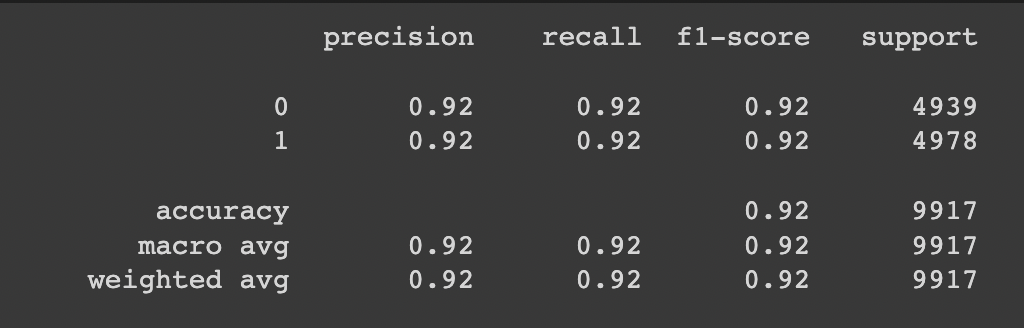
\includegraphics[scale=0.6]{figuras/as-resultados-2.png}
    % \caption[Así aparece el rótulo en el índice]{Así aparece el rótulo en el texto.}
    \caption[Análisis de Sentimiento - Resultados - Métricas de clasificación]{\textbf{Métricas de clasificación obtenidas en el modelo. Fuente: Imagen propia}}
    \label{fig-as-resultados-2}
\end{figure}

\begin{figure}[ht!]
    \centering
    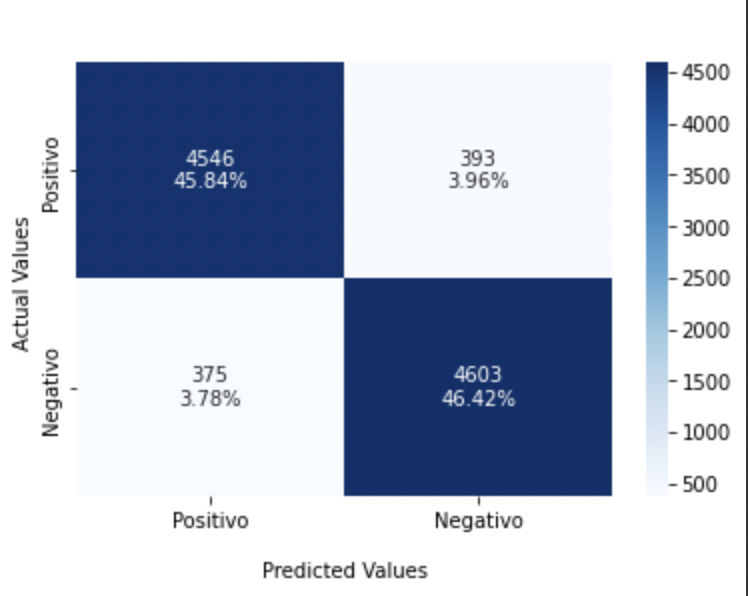
\includegraphics[scale=0.6]{figuras/as-resultados-3.png}
    % \caption[Así aparece el rótulo en el índice]{Así aparece el rótulo en el texto.}
    \caption[Análisis de Sentimiento - Resultados - Matriz de confusión]{\textbf{Matriz de confusión resultado de la evaluación del modelo. Fuente: Imagen propia}}
    \label{fig-as-resultados-3}
\end{figure}
